\clearpage
\appendix
\maketitlesupplementary

\section{Datasets}
\label{app:dataset_details}
We evaluate the proposed method on four datasets covering substantially
different video-segmentation settings: object transformation in VOST,
camouflaged objects in CAMotion, colonoscopy in SUN-SEG, and thyroid
ultrasound in VTUS.
This diversity allows us to assess frame selection
under different appearance changes, object visibility, imaging
modalities, and mask-propagation failures.

We preserve the original training and validation splits of each dataset.
To increase the number of training samples, long training videos are
divided into shorter overlapping clips, while VOST videos are used
without division. Validation videos are kept unchanged. The dataset sizes
and clip-generation settings are reported in
Table~\ref{tab:app_dataset_statistics}.

\begin{table}[!h]
\caption{Dataset splits and temporal partitioning used to construct the
training clips. Window and stride are measured in frames. Dashes indicate
that the original videos are used without partitioning.}
\label{tab:app_dataset_statistics}

\centering
\setlength{\tabcolsep}{2.2pt}
{\small
\begin{tabular}{@{}lcccccc@{}}
\toprule
\textbf{Dataset}
&
\multicolumn{2}{c}{\textbf{Original}}
&
\multicolumn{2}{c}{\textbf{Partitioning}}
&
\multicolumn{2}{c}{\textbf{Final}}
\\
\cmidrule(lr){2-3}
\cmidrule(lr){4-5}
\cmidrule(l){6-7}
&
\textbf{Train}
&
\textbf{Val.}
&
\textbf{Window}
&
\textbf{Stride}
&
\textbf{Train}
&
\textbf{Val.}
\\
\midrule
VOST
& 572 & 71
& -- & --
& 572 & 71
\\
SUN-SEG
& 112 & 37
& 100 & 10
& 917 & 37
\\
VTUS
& 70 & 30
& 50 & 5
& 686 & 30
\\
CAMOtion
& 359 & 115
& 100 & 10
& 528 & 115
\\
\bottomrule
\end{tabular}
}

\end{table}


For each training clip and validation video, we define ten uniformly
spaced temporal locations. The first receives the initial ground-truth
mask prompt, and the remaining nine are correction candidates. These
locations only determine where prompts can be placed; SAM2 propagates
over the entire sequence, and mIoU is computed over all frames in that
sequence.

\section{Additional implementation details}

\subsection{Promptable segmentation model configurations}

We use a frozen SAM2.1 Hiera-Tiny model with an internal image size of
\(512\times512\) to reduce propagation time without a noticeable loss in
segmentation accuracy.

We use ground-truth masks as the initial and corrective prompts. A
ground-truth mask represents an ideal expert correction after the system
defers a frame for annotation. This removes variation caused by prompt
quality and allows the experiments to isolate the decisions of whether
to request correction, how many frames to correct, and which frames to
select.

\subsection{Architectural details}

\paragraph{Feature representation and encoder.}
For each sampled frame location, we use the mask-memory feature map produced
by the frozen SAM2.1 memory encoder. This representation jointly encodes the
frame appearance and its current predicted mask, and is used by SAM2 to
condition subsequent mask propagation.

Each mask-memory feature map is adaptively average-pooled to a \(4\times4\)
grid, yielding 16 spatial tokens with 64 channels. The tokens are projected to
128 dimensions, combined with learned spatial positional embeddings, and
processed by one four-head spatial Transformer layer. Spatial mean pooling
then produces one representation per frame. After adding learned temporal
positional embeddings, two four-head temporal Transformer layers exchange
information across the sampled video sequence, producing a contextualized
128-dimensional representation \(\mathbf{h}_i\) for each location. The frame
selector and cardinality model use independently trained encoders with this
architecture and do not share parameters.

\paragraph{Multi-frame selection head.}
The selector uses single-head soft cross-attention, with each candidate frame
as the query and the prompted and previously selected frames as keys and
values. The resulting 128-dimensional context vector is concatenated with the
128-dimensional candidate representation and a learned 128-dimensional
embedding of the requested cardinality. The resulting 384-dimensional vector
is processed by layer normalization and a two-layer MLP with dimensions
\(384\rightarrow128\rightarrow1\), using GELU activation and dropout 0.1.
Previously prompted and selected frames are masked. The next frame is sampled
categorically during training and selected greedily during inference.

\begin{table*}[t]
\caption{Variable-cardinality frame selection under maximum correction budgets
\(K_{\max}\in\{2,3,4,5,6\}\) at \(\alpha=0.01\). For each method and dataset,
we report video-level segmentation quality (\(\mathrm{mIoU}\uparrow\)) and the
mean number of selected correction frames (\(\bar{k}\downarrow\)). Boldface
denotes our method.}
\label{tab:app_variable_cardinality}

\centering
\small
\setlength{\tabcolsep}{3.2pt}
\begin{tabular}{@{}llcccccccc@{}}
\toprule
& & \multicolumn{2}{c}{\textbf{VOST}} & \multicolumn{2}{c}{\textbf{CAMOtion}} & \multicolumn{2}{c}{\textbf{SUN-SEG}} & \multicolumn{2}{c}{\textbf{VTUS}} \\
\cmidrule(lr){3-4} \cmidrule(lr){5-6} \cmidrule(lr){7-8} \cmidrule(l){9-10}
\textbf{K} & \textbf{Method} & mIoU & $\bar{k}$ & mIoU & $\bar{k}$ & mIoU & $\bar{k}$ & mIoU & $\bar{k}$ \\
\midrule

2 & LECODU & 0.622 & 2.00 & 0.828 & 1.01 & 0.802 & 2.00 & 0.739 & 2.00 \\
2 & Top-\(k\) (\(x\)) & 0.638 & 1.57 & 0.831 & 0.74 & 0.813 & 1.32 & 0.756 & 1.80 \\
2 & \textbf{Ours} & \textbf{0.671} & \textbf{2.00} & \textbf{0.838} & \textbf{0.93} & \textbf{0.830} & \textbf{1.29} & \textbf{0.777} & \textbf{1.97} \\
\midrule
3 & LECODU & 0.642 & 3.00 & 0.830 & 0.95 & 0.814 & 2.12 & 0.758 & 3.00 \\
3 & Top-\(k\) (\(x\)) & 0.668 & 2.33 & 0.832 & 0.89 & 0.827 & 1.59 & 0.774 & 2.37 \\
3 & \textbf{Ours} & \textbf{0.686} & \textbf{2.44} & \textbf{0.841} & \textbf{1.01} & \textbf{0.841} & \textbf{1.60} & \textbf{0.797} & \textbf{2.73} \\
\midrule
4 & LECODU & 0.658 & 3.21 & 0.837 & 1.28 & 0.836 & 2.01 & 0.755 & 3.26 \\
4 & Top-\(k\) (\(x\)) & 0.662 & 2.82 & 0.838 & 1.30 & 0.842 & 1.80 & 0.795 & 2.90 \\
4 & \textbf{Ours} & \textbf{0.699} & \textbf{2.56} & \textbf{0.847} & \textbf{1.19} & \textbf{0.850} & \textbf{1.71} & \textbf{0.819} & \textbf{2.81} \\
\midrule
5 & LECODU & 0.670 & 4.63 & 0.841 & 1.36 & 0.847 & 2.52 & 0.803 & 3.86 \\
5 & Top-\(k\) (\(x\)) & 0.671 & 3.50 & 0.840 & 0.94 & 0.845 & 2.05 & 0.804 & 3.00 \\
5 & \textbf{Ours} & \textbf{0.706} & \textbf{3.73} & \textbf{0.849} & \textbf{1.13} & \textbf{0.866} & \textbf{2.24} & \textbf{0.837} & \textbf{4.20} \\
\midrule
6 & LECODU & 0.684 & 4.96 & 0.849 & 1.22 & 0.855 & 2.26 & 0.819 & 4.42 \\
6 & Top-\(k\) (\(x\)) & 0.680 & 4.09 & 0.842 & 1.33 & 0.852 & 2.24 & 0.811 & 4.47 \\
6 & \textbf{Ours} & \textbf{0.715} & \textbf{3.67} & \textbf{0.855} & \textbf{1.45} & \textbf{0.877} & \textbf{2.32} & \textbf{0.847} & \textbf{4.07} \\
\bottomrule
\end{tabular}

\end{table*}


\paragraph{Cardinality head.}
The cardinality model mean-pools its encoded frame representations to obtain a
128-dimensional video-level vector. This vector is processed by layer
normalization and a two-layer MLP with dimensions
\(128\rightarrow128\rightarrow(K+1)\), using GELU activation and dropout 0.1.
The outputs represent non-deferral and cardinalities \(1,\ldots,K\). The frame
selector is frozen during cardinality-model training.

The complete deferral decision, including cardinality prediction and frame selection, takes approximately \(30\,\mathrm{ms}\) per video, excluding SAM2 propagation.

\section{Additional baseline details}

We adapt baselines from learning to defer and video frame selection. All
baselines use the same frozen SAM2.1 Hiera-Tiny model, sampled prompt
locations, and ground-truth mask prompts. The first location provides the
initial prompt, while the remaining locations are eligible for additional
expert prompts. The methods differ in how they determine the prompt
cardinality \(k\) and select the corresponding frames.

\subsection{Reference policies.}
The non-deferral policy requests no additional prompt (\(k=0\)) and retains
the initial SAM2 propagation. For a given \(k>0\), the minimum-IoU policy
selects the \(k\) eligible frames with the lowest frame-level IoU. This
approximates an expert visually inspecting the propagation and prompting the
frames that appear most erroneous.

For fixed-cardinality evaluation, \(k\) is specified in advance. The random
policy uniformly samples a \(k\)-frame subset without replacement, while the
oracle selects the subset of size \(k\) that produces the highest video-level
mIoU. For variable-cardinality evaluation, the random policy first samples
\(k\) uniformly from \(\{0,\ldots,K\}\) and then samples \(k\) eligible frames.
The oracle jointly selects the cardinality and frame subset with the lowest
cost \(1-\operatorname{mIoU}+\alpha k\). In both settings, the oracle is
computed by evaluating all eligible combinations only to compare our method
with the best achievable performance; this exhaustive search is not required
during training or inference.

\subsection{Learning-to-defer adaptations.}
All learning-to-defer baselines use the same inputs and
cardinality architecture as our method.
Only their output spaces and training losses are changed to follow the
corresponding original formulations.

LECODU and Adaptive Top-$k(x)$
were originally formulated for classification with multiple users or experts.
We treat each eligible frame location as a deferral action, where selecting it
requests an expert mask prompt. In our LECODU adaptation, the predicted number
of users determines \(k\), after which \(k\) eligible frames are sampled
uniformly. Adaptive Top-$k(x)$ predicts \(k\), estimates the utility of
prompting each frame independently, and selects the \(k\) highest-ranked
frames.

L2RP was originally designed for promptable video
segmentation. We adapt it to our inputs and
cardinality architecture while retaining its original loss and output
space. It therefore decides between retaining the current propagation and
requesting one expert prompt at a selected frame, supporting only
\(k\in\{0,1\}\).

\begin{table*}[t]
\caption{Fixed-cardinality frame selection for \(k\in\{2,3,4\}\). Batch methods select all \(k\) frames before a single propagation, whereas sequential methods select and propagate one correction at a time. We report video-level mIoU; the oracle gives the best frame subset for each \(k\).}
\label{tab:fixed_cardinality_appendix}

\centering
\small
\setlength{\tabcolsep}{3.2pt}
\begin{tabular}{@{}llcccccccccccc@{}}
\toprule
& & \multicolumn{3}{c}{\textbf{VOST}} & \multicolumn{3}{c}{\textbf{CAMotion}} & \multicolumn{3}{c}{\textbf{SUN-SEG}} & \multicolumn{3}{c}{\textbf{VTUS}} \\
\cmidrule(lr){3-5} \cmidrule(lr){6-8} \cmidrule(lr){9-11} \cmidrule(l){12-14}
\textbf{Method} & \textbf{Selection} & \(k{=}2\) & \(k{=}3\) & \(k{=}4\) & \(k{=}2\) & \(k{=}3\) & \(k{=}4\) & \(k{=}2\) & \(k{=}3\) & \(k{=}4\) & \(k{=}2\) & \(k{=}3\) & \(k{=}4\) \\
\midrule
Random frames & Batch & 0.584 & 0.613 & 0.632 & 0.825 & 0.831 & 0.845 & 0.766 & 0.787 & 0.802 & 0.693 & 0.727 & 0.760 \\
Worst-IoU frames & Batch & 0.591 & 0.647 & 0.663 & 0.836 & 0.843 & 0.842 & 0.787 & 0.791 & 0.818 & 0.721 & 0.748 & 0.772 \\
HSVA (2023) & Batch & 0.635 & 0.663 & 0.679 & 0.837 & 0.844 & 0.845 & 0.792 & 0.828 & 0.830 & 0.770 & 0.781 & 0.794 \\
IVOS-W (2021) & Sequential & 0.606 & 0.655 & 0.675 & 0.838 & 0.845 & 0.848 & 0.791 & 0.818 & 0.838 & 0.720 & 0.769 & 0.796 \\
EVA-VOS (2024) & Sequential & 0.629 & 0.667 & 0.681 & 0.846 & 0.848 & 0.854 & 0.800 & 0.825 & 0.852 & 0.763 & 0.786 & 0.810 \\
Top-\(k\) (2025) & Batch & 0.643 & 0.670 & 0.683 & 0.844 & 0.847 & 0.850 & 0.811 & 0.829 & 0.845 & 0.750 & 0.772 & 0.804 \\
\textbf{Ours} & \textbf{Batch} & \textbf{0.671} & \textbf{0.688} & \textbf{0.701} & \textbf{0.849} & \textbf{0.852} & \textbf{0.859} & \textbf{0.844} & \textbf{0.862} & \textbf{0.868} & \textbf{0.787} & \textbf{0.799} & \textbf{0.820} \\
\midrule
\emph{Oracle} & \emph{Batch} & \emph{0.695} & \emph{0.712} & \emph{0.721} & \emph{0.854} & \emph{0.859} & \emph{0.862} & \emph{0.860} & \emph{0.875} & \emph{0.881} & \emph{0.813} & \emph{0.828} & \emph{0.835} \\
\bottomrule
\end{tabular}

\end{table*}


\begin{figure*}[t]
    \centering
    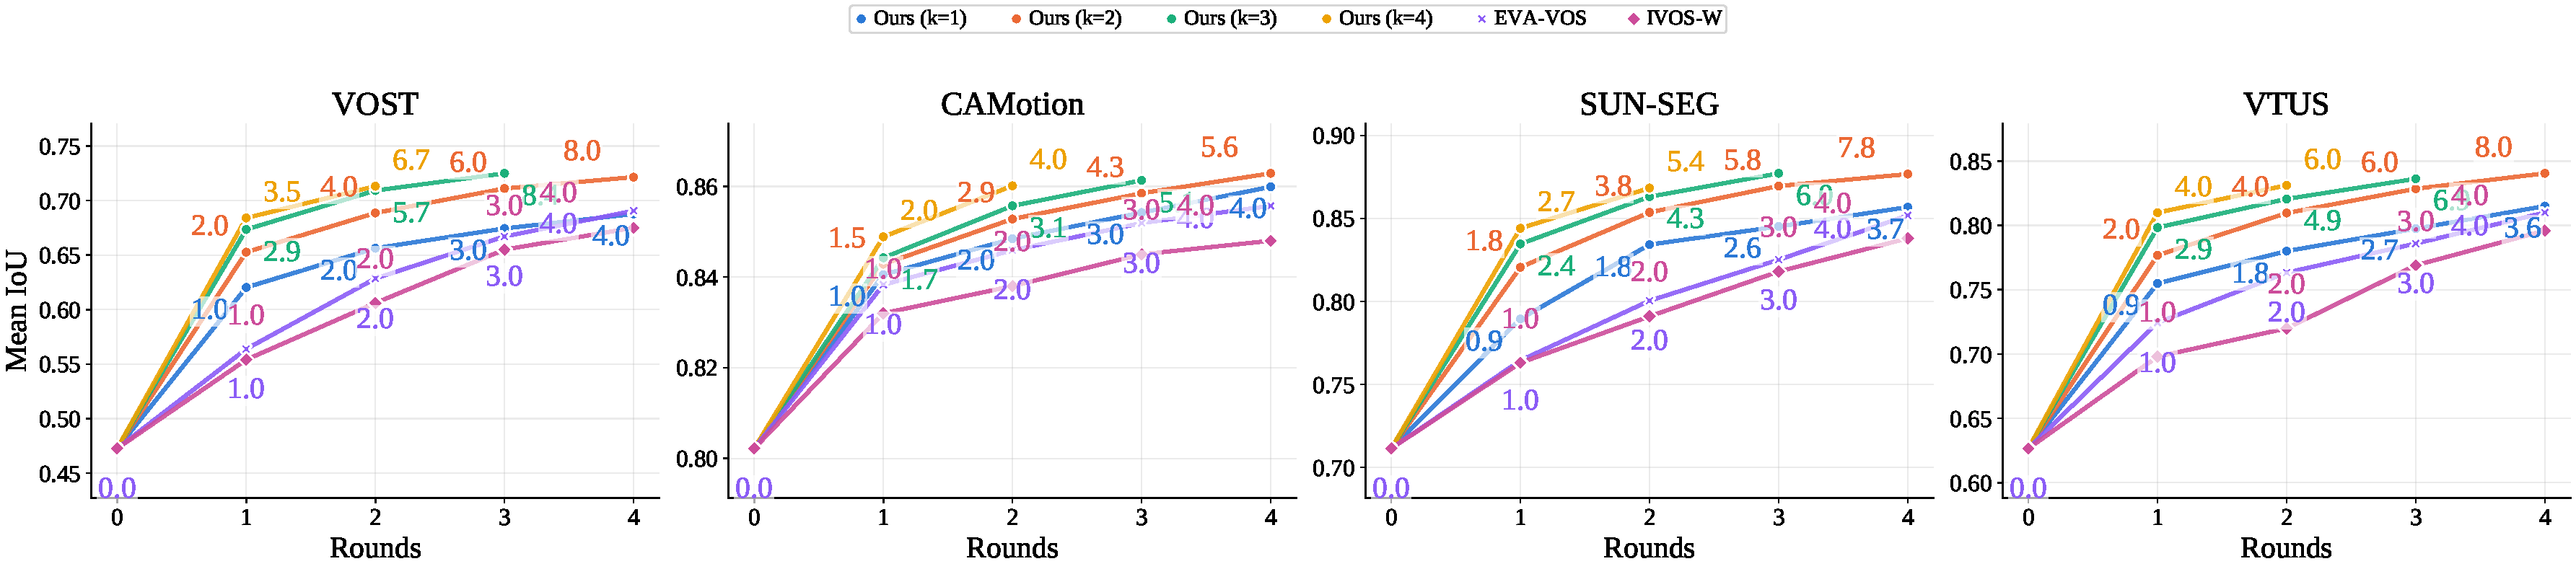
\includegraphics[width=\textwidth]
    {Figures/iterative_iou_meank_by_round_maxk1to4_all_datasets.pdf}
    \caption{Mean IoU over corrective-prompting rounds on all four datasets
    at \(\alpha=0.001\). Our models with maximum cardinality
    \(K\in\{1,2,3,4\}\) select multiple correction frames as a batch in each
    round, whereas EVA-VOS and IVOS-W select one frame per round. After each
    round, the selected frames are prompted and the full video is
    re-propagated. Point labels indicate the mean cumulative number of
    selected correction frames.}
    \label{fig:iterative_all_datasets}
\end{figure*}

\subsection{Video frame-selection adaptations.}
Lazy-XMem, HVSA,
EVA-VOS, and IVOS-W use different
criteria for determining when or where annotations should be requested. We
retain their triggering or frame-selection procedures while using the same
frozen SAM2.1 model and eligible frame locations. Lazy-XMem uses prediction
uncertainty to trigger a prompt; HVSA selects frames using uncertainty and
diversity; EVA-VOS uses its frame-selection component; and IVOS-W uses its
learned frame-recommendation policy.

The original HVSA framework performs video-specific test-time fine-tuning
after acquiring annotations. Our adaptation uses only its frame-selection
procedure and does not retrain the segmentation model. Instead, selected
frames receive ground-truth mask prompts and the frozen SAM2.1 model propagates
the updated segmentation. Further, sequential methods re-propagate after each
prompt before selecting the next frame, whereas batch methods select all
\(k\) frames from the current propagation and apply their prompts together.

\section{Additional results}

\subsection{Variable cardinality for different maximum budgets}
The main experiments use \(K=4\) additional corrections. Table~\ref{tab:app_variable_cardinality} extends this analysis to
\(K_{\max}\in\{2,3,4,5,6\}\) at \(\alpha=0.01\). Our method achieves
the highest mIoU across all datasets and correction limits.

\subsection{Fixed-cardinality frame selection for different budgets}

Table~\ref{tab:fixed_cardinality_appendix} shows that our method achieves the
highest non-oracle mIoU across all datasets and
\(k\in\{2,3,4\}\). The gains are particularly clear on VOST, SUN-SEG,
and VTUS, while competing methods perform more similarly on CAMotion.
This indicates that our selector identifies more effective sets of
correction frames under the same fixed expert budget.

\subsection{Iterative application across datasets}
Figure~\ref{fig:iterative_all_datasets} extends the SUN-SEG analysis in
the main paper to all four datasets. We use \(\alpha=0.001\) so that the
policy continues to request useful corrections over multiple rounds,
rather than quickly selecting \(k=0\) as segmentation quality improves.
This setting also provides a closer comparison with EVA-VOS and IVOS-W,
which focus on frame selection without accounting for expert cost. The results show that batch selection can obtain gains
comparable to multiple sequential interventions in fewer interaction
rounds, although the benefit varies with the dataset and maximum
cardinality \(K\)

\subsection{Results for different expert costs}

The main paper reports results at \(\alpha=0.01\) and visualises the
quality--cost trade-off across additional expert costs.  Here, we
provide the exact values corresponding to the curves shown in the main
figure. Each table entry reports the video-level mIoU and average
selected cardinality, \((\mathrm{mIoU}, \widehat{k})\), for
a given value of \(\alpha\).

\begin{table*}[t]
\caption{Ablation on the expert costs \(\alpha\) on VOST and
CAMotion. Each entry reports
\((\mathrm{mIoU},\,\widehat{k})\), where
\(\widehat{k}\) is the mean number of selected correction
frames. Continued in Table~\ref{tab:alpha_sweep_sunseg_vtus}.}
\label{tab:alpha_sweep_vost_camotion}

\centering
\setlength{\tabcolsep}{4pt}
\renewcommand{\arraystretch}{1.08}
{\small
\begin{tabular}{@{}c*{6}{c}@{}}
\toprule
&
\multicolumn{3}{c}{\textbf{VOST}}
&
\multicolumn{3}{c}{\textbf{CAMotion}}
\\
\cmidrule(lr){2-4}
\cmidrule(lr){5-7}

\(\boldsymbol{\alpha}\)
& \textbf{Ours}
& \textbf{Top-\(k(x)\)}
& \textbf{LECODU}
& \textbf{Ours}
& \textbf{Top-\(k(x)\)}
& \textbf{LECODU}
\\
\midrule

0
& \((0.705,\,3.97)\)
& \((0.679,\,4.00)\)
& \((0.670,\,4.00)\)
& \((0.859,\,3.99)\)
& \((0.850,\,4.00)\)
& \((0.847,\,4.00)\)
\\

0.005
& \((0.702,\,3.47)\)
& \((0.663,\,2.93)\)
& \((0.670,\,4.00)\)
& \((0.850,\,2.03)\)
& \((0.844,\,1.77)\)
& \((0.843,\,2.07)\)
\\

0.01
& \((0.699,\,2.56)\)
& \((0.662,\,2.82)\)
& \((0.658,\,3.21)\)
& \((0.847,\,1.19)\)
& \((0.838,\,1.30)\)
& \((0.837,\,1.28)\)
\\

0.015
& \((0.685,\,2.34)\)
& \((0.649,\,2.46)\)
& \((0.655,\,3.11)\)
& \((0.838,\,0.72)\)
& \((0.830,\,0.63)\)
& \((0.825,\,0.52)\)
\\

0.02
& \((0.673,\,2.03)\)
& \((0.644,\,2.26)\)
& \((0.652,\,2.91)\)
& \((0.836,\,0.67)\)
& \((0.826,\,0.47)\)
& \((0.820,\,0.14)\)
\\

0.05
& \((0.622,\,1.11)\)
& \((0.607,\,1.39)\)
& \((0.610,\,1.40)\)
& \((0.817,\,0.03)\)
& \((0.818,\,0.04)\)
& \((0.802,\,0.00)\)
\\

0.1
& \((0.609,\,0.97)\)
& \((0.554,\,0.63)\)
& \((0.531,\,0.53)\)
& \((0.817,\,0.03)\)
& \((0.815,\,0.01)\)
& \((0.802,\,0.00)\)
\\

0.15
& \((0.522,\,0.30)\)
& \((0.511,\,0.34)\)
& \((0.476,\,0.01)\)
& \((0.815,\,0.01)\)
& \((0.802,\,0.00)\)
& \((0.802,\,0.00)\)
\\

0.2
& \((0.484,\,0.04)\)
& \((0.506,\,0.24)\)
& \((0.473,\,0.00)\)
& \((0.815,\,0.01)\)
& \((0.802,\,0.00)\)
& \((0.802,\,0.00)\)
\\

0.3
& \((0.473,\,0.00)\)
& \((0.479,\,0.06)\)
& \((0.473,\,0.00)\)
& \((0.802,\,0.00)\)
& \((0.802,\,0.00)\)
& \((0.802,\,0.00)\)
\\

0.4
& \((0.473,\,0.00)\)
& \((0.473,\,0.01)\)
& \((0.473,\,0.00)\)
& \((0.802,\,0.00)\)
& \((0.802,\,0.00)\)
& \((0.802,\,0.00)\)
\\

\bottomrule
\end{tabular}
}

\end{table*}


\begin{table*}[t]
\caption{Ablation on the expert costs \(\alpha\) on SUN-SEG and
VTUS, continued from Table~\ref{tab:alpha_sweep_vost_camotion}.}
\label{tab:alpha_sweep_sunseg_vtus}

\centering
\setlength{\tabcolsep}{4pt}
\renewcommand{\arraystretch}{1.08}
{\small
\begin{tabular}{@{}c*{6}{c}@{}}
\toprule
&
\multicolumn{3}{c}{\textbf{SUN-SEG}}
&
\multicolumn{3}{c}{\textbf{VTUS}}
\\
\cmidrule(lr){2-4}
\cmidrule(lr){5-7}

\(\boldsymbol{\alpha}\)
& \textbf{Ours}
& \textbf{Top-\(k(x)\)}
& \textbf{LECODU}
& \textbf{Ours}
& \textbf{Top-\(k(x)\)}
& \textbf{LECODU}
\\
\midrule

0
& \((0.868,\,4.00)\)
& \((0.853,\,4.00)\)
& \((0.849,\,4.00)\)
& \((0.820,\,4.00)\)
& \((0.804,\,4.00)\)
& \((0.780,\,4.00)\)
\\

0.005
& \((0.866,\,2.73)\)
& \((0.852,\,3.11)\)
& \((0.843,\,3.03)\)
& \((0.820,\,3.97)\)
& \((0.802,\,3.73)\)
& \((0.768,\,3.64)\)
\\

0.01
& \((0.850,\,1.71)\)
& \((0.842,\,1.80)\)
& \((0.836,\,2.01)\)
& \((0.819,\,2.81)\)
& \((0.795,\,2.90)\)
& \((0.755,\,3.26)\)
\\

0.015
& \((0.848,\,1.55)\)
& \((0.838,\,1.71)\)
& \((0.828,\,1.86)\)
& \((0.809,\,2.35)\)
& \((0.759,\,1.90)\)
& \((0.737,\,2.22)\)
\\

0.02
& \((0.847,\,1.41)\)
& \((0.825,\,1.27)\)
& \((0.814,\,1.46)\)
& \((0.798,\,2.00)\)
& \((0.742,\,1.73)\)
& \((0.733,\,2.14)\)
\\

0.05
& \((0.830,\,1.00)\)
& \((0.803,\,0.86)\)
& \((0.788,\,1.03)\)
& \((0.728,\,0.90)\)
& \((0.717,\,0.80)\)
& \((0.717,\,1.47)\)
\\

0.1
& \((0.795,\,0.65)\)
& \((0.789,\,0.68)\)
& \((0.755,\,0.49)\)
& \((0.694,\,0.50)\)
& \((0.706,\,0.53)\)
& \((0.652,\,0.13)\)
\\

0.15
& \((0.768,\,0.22)\)
& \((0.780,\,0.62)\)
& \((0.750,\,0.46)\)
& \((0.676,\,0.23)\)
& \((0.663,\,0.23)\)
& \((0.627,\,0.00)\)
\\

0.2
& \((0.725,\,0.03)\)
& \((0.770,\,0.46)\)
& \((0.721,\,0.03)\)
& \((0.651,\,0.07)\)
& \((0.660,\,0.13)\)
& \((0.627,\,0.00)\)
\\

0.3
& \((0.725,\,0.03)\)
& \((0.747,\,0.16)\)
& \((0.711,\,0.00)\)
& \((0.642,\,0.03)\)
& \((0.650,\,0.07)\)
& \((0.627,\,0.00)\)
\\

0.4
& \((0.725,\,0.03)\)
& \((0.745,\,0.08)\)
& \((0.711,\,0.00)\)
& \((0.633,\,0.03)\)
& \((0.627,\,0.00)\)
& \((0.627,\,0.00)\)
\\

\bottomrule
\end{tabular}
}

\end{table*}


\subsection{Qualitative results}

Figures~\ref{fig:vost_qualitative}--\ref{fig:vtus_qualitative} present qualitative comparisons on VOST, CAMotion, SUN-SEG, and VTUS using examples spanning different levels of initial propagation quality. Across these cases, our method selects correction cardinalities and frame sets that achieve higher final IoU and lower system cost than Top-$k(x)$. The examples further illustrate complementary frame selection in difficult videos and the avoidance of unnecessary corrections when the initial propagation is already reliable.

\begin{figure*}[t]
    \centering
    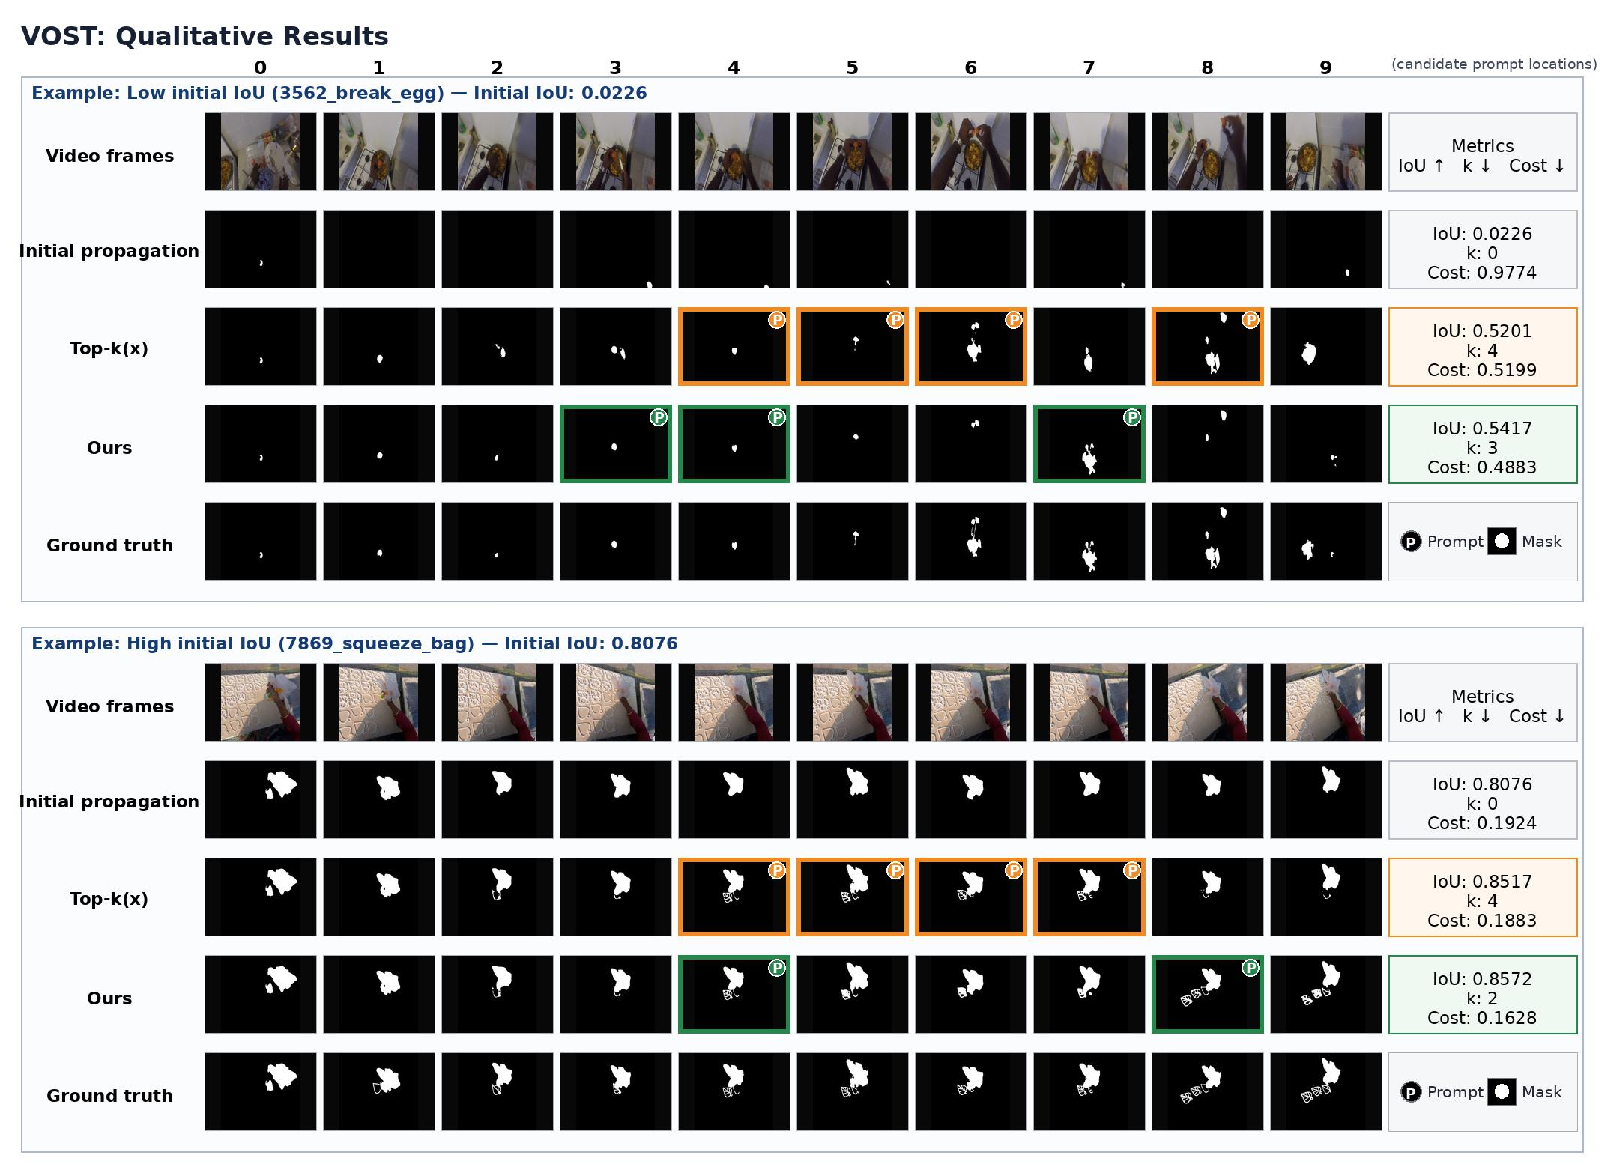
\includegraphics[width=\textwidth]{Figures/vost_comparison_grid.pdf}
    \caption{Qualitative comparison on VOST, which contains substantial object appearance and shape transformations. The examples show an egg being broken and a bag being squeezed, where deformation makes mask propagation challenging. The Top-$k(x)$ and Ours rows show the masks obtained after applying all selected corrective prompts and re-propagating the video. In the low-initial-IoU example, our method achieves higher final IoU using fewer prompts and lower system cost. In the high-initial-IoU example, it avoids unnecessary corrections while obtaining slightly higher IoU and lower cost. Coloured borders and prompt markers indicate the selected correction frames.}
    \label{fig:vost_qualitative}
\end{figure*}

\begin{figure*}[t]
    \centering
    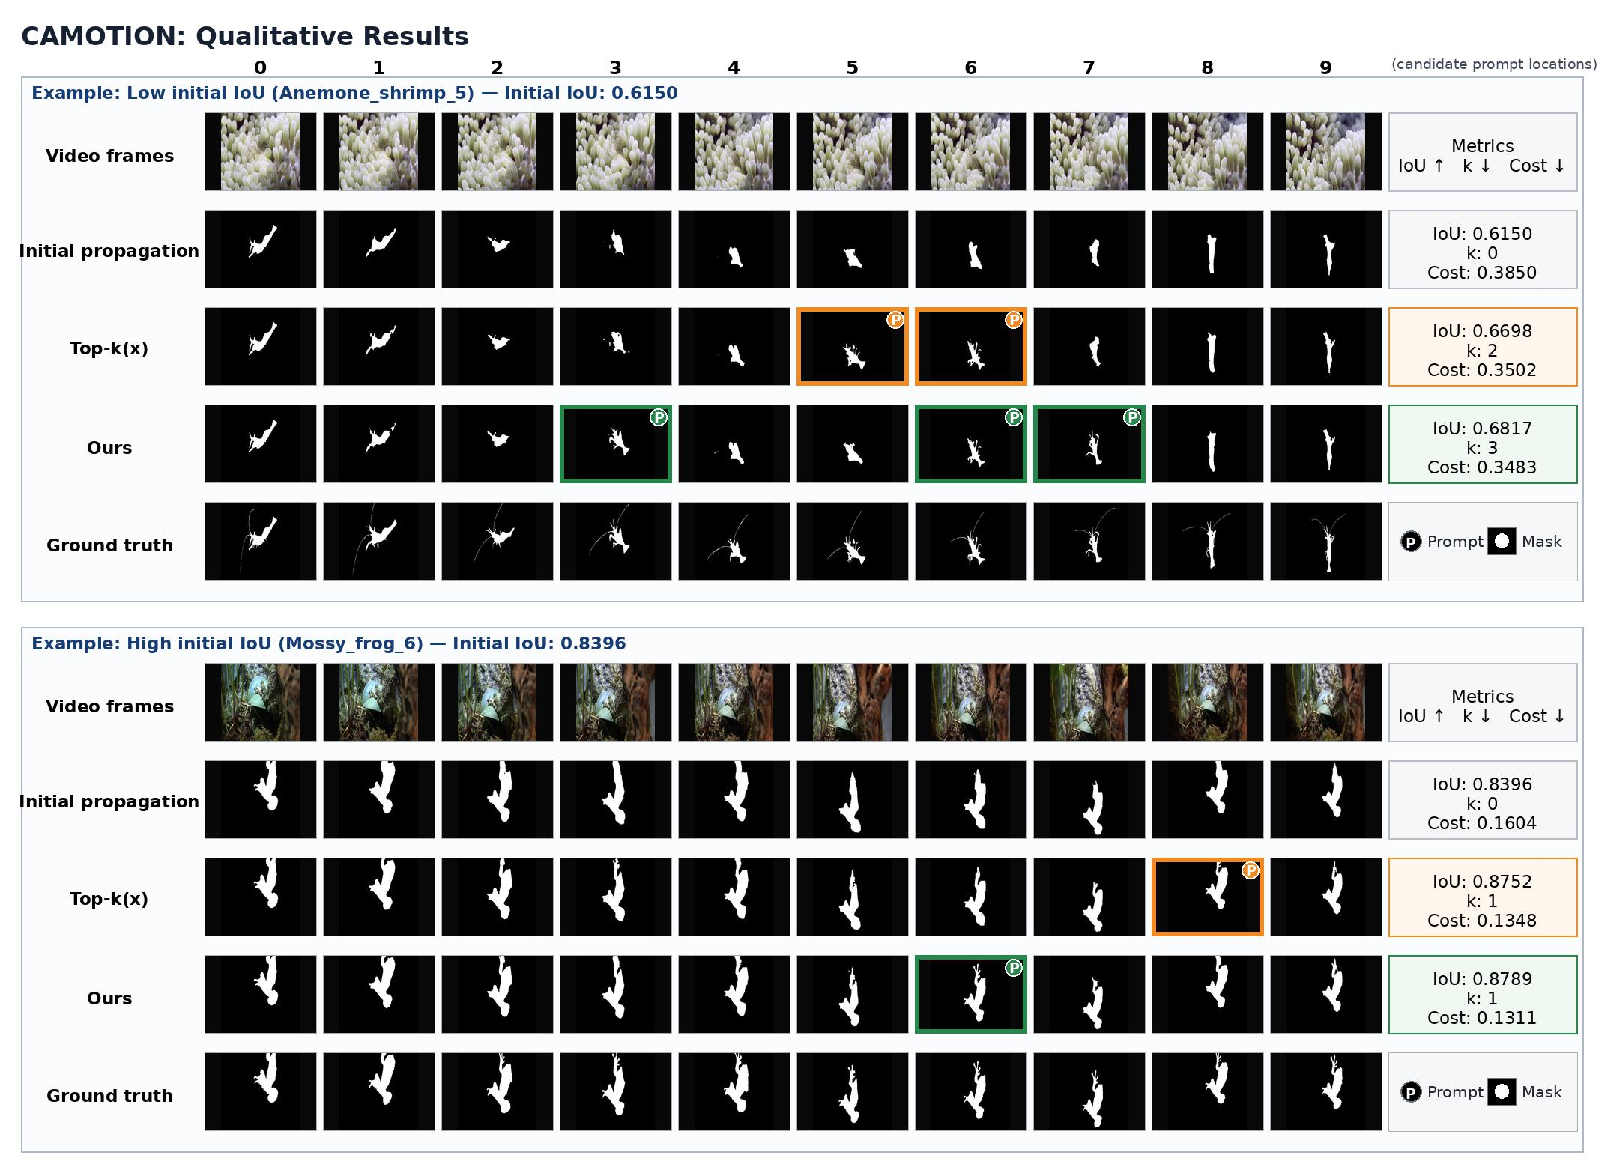
\includegraphics[width=\textwidth]
    {Figures/camotion_comparison_grid.pdf}
    \caption{Qualitative comparison on CAMotion, where foreground objects are difficult to distinguish from their surrounding backgrounds. The examples show an anemone shrimp with relatively low initial IoU and a mossy frog with high initial IoU. The Top-$k(x)$ and Ours rows show the masks obtained after applying the selected corrective prompts and re-propagating the video. In the low-initial-IoU example, our method achieves higher IoU and lower system cost by selecting three complementary correction frames. In the high-initial-IoU example, both methods request one correction, while our selected frame yields slightly higher IoU and lower cost. Coloured borders and prompt markers indicate the selected correction frames.}
    \label{fig:camotion_qualitative}
\end{figure*}

\begin{figure*}[t]
    \centering
    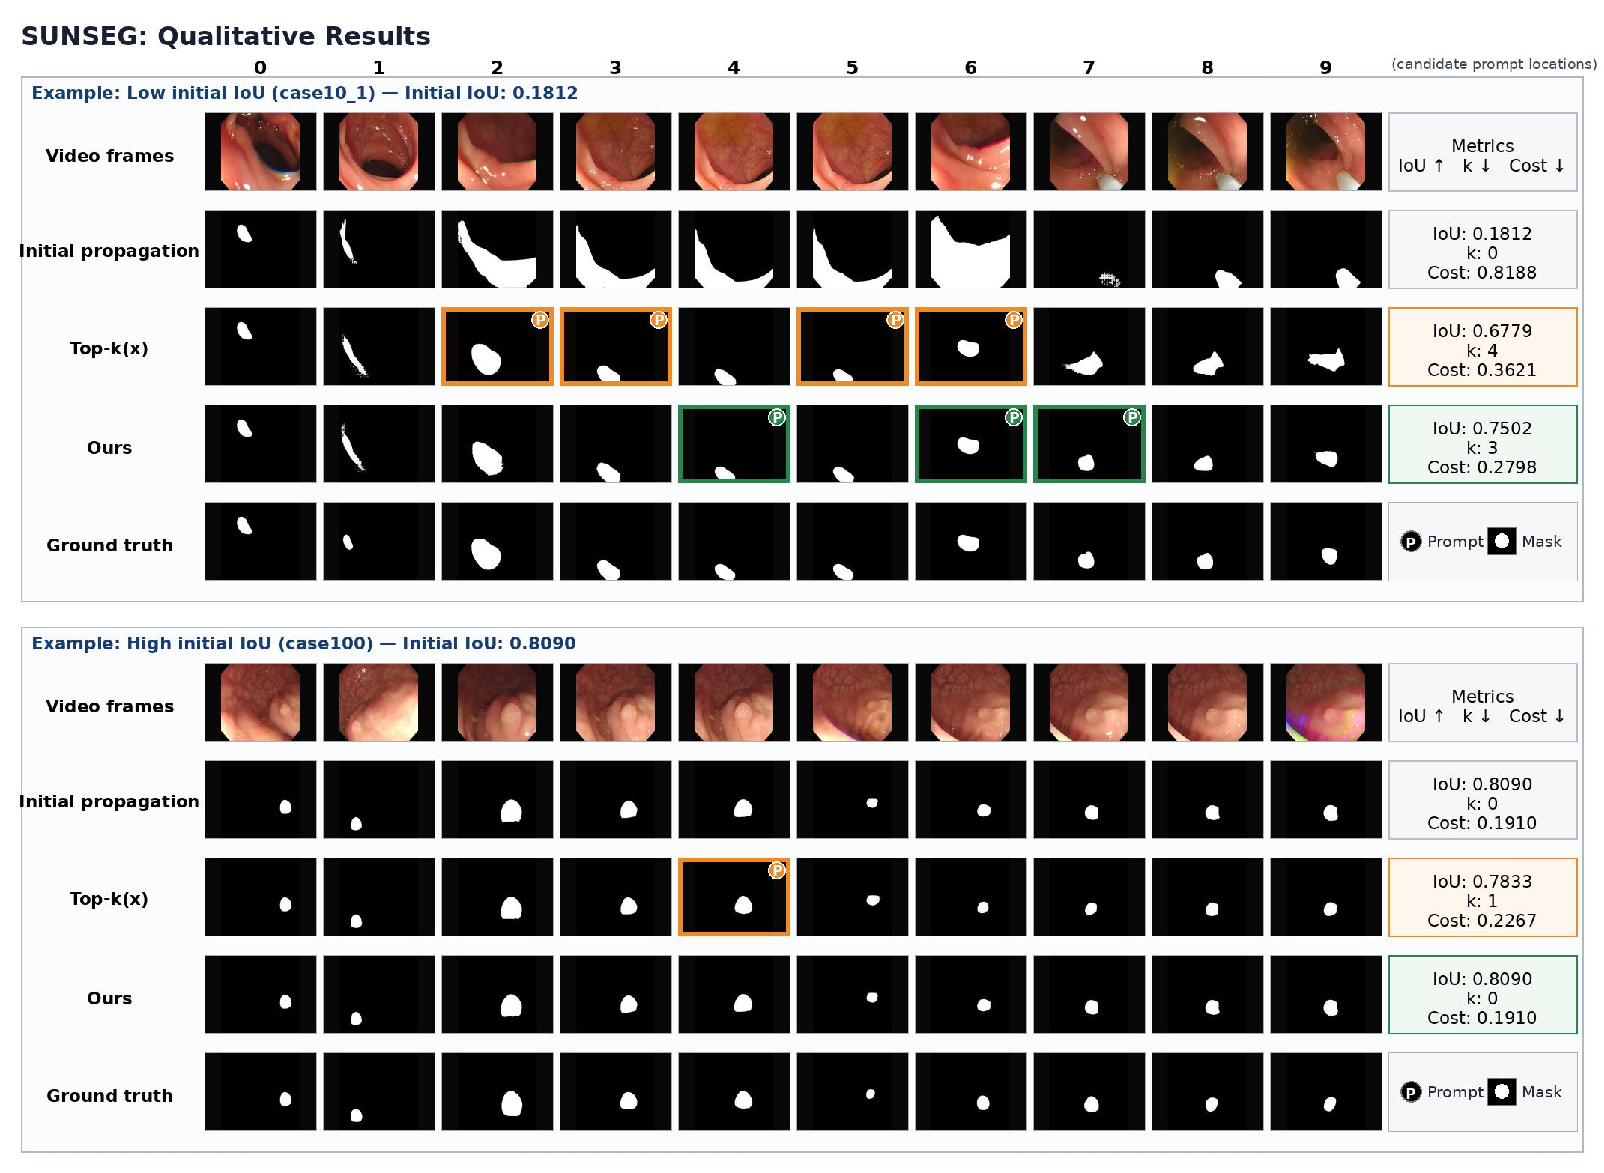
\includegraphics[width=\textwidth]
    {Figures/sunseg_comparison_grid.pdf}
    \caption{Qualitative comparison on SUN-SEG, where polyp appearance, scale, and viewpoint can vary substantially across colonoscopy frames. The Top-$k(x)$ and Ours rows show the masks obtained after applying the selected corrective prompts and re-propagating the video. In the low-initial-IoU example, our method selects three corrective frames and achieves substantially higher IoU with lower system cost than Top-$k(x)$, which requests four prompts. In the high-initial-IoU example, our method retains the initial propagation with \(k=0\), whereas Top-$k(x)$ requests an unnecessary correction that reduces IoU and increases system cost. Coloured borders and prompt markers indicate the selected correction frames.}
    \label{fig:sunseg_qualitative}
\end{figure*}

\begin{figure*}[t]
    \centering
    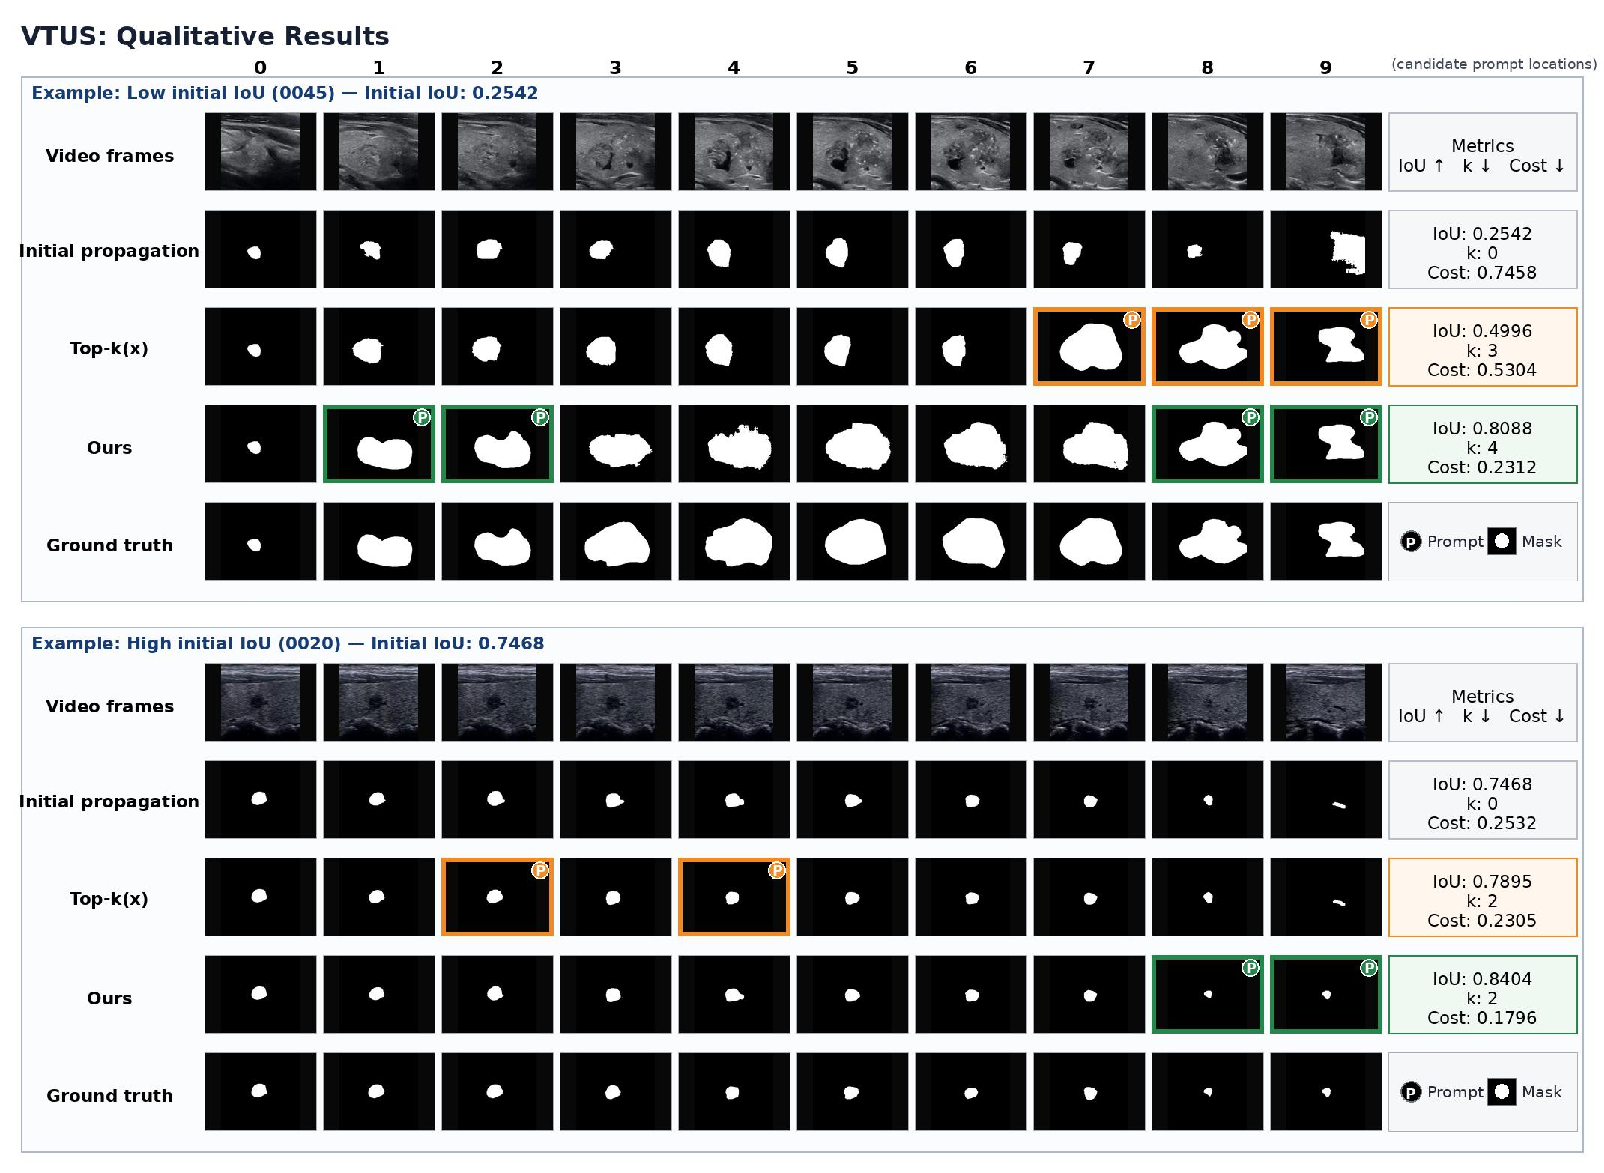
\includegraphics[width=\textwidth]
    {Figures/vtus_comparison_grid.pdf}
    \caption{Qualitative comparison on VTUS, where thyroid nodules exhibit low contrast, ambiguous boundaries, and substantial variation in appearance across ultrasound frames. The Top-$k(x)$ and Ours rows show the masks obtained after applying the selected corrective prompts and re-propagating the video. In the low-initial-IoU example, our method selects four complementary correction frames and substantially improves IoU while achieving a much lower system cost than Top-$k(x)$. In the high-initial-IoU example, both methods request two corrections, but our selected frames yield higher IoU and lower system cost. Coloured borders and prompt markers indicate the selected correction frames.}
    \label{fig:vtus_qualitative}
\end{figure*}
